\documentclass[a5paper,openany,10pt]{book}
\usepackage[utf8]{inputenc}
\usepackage[english,russian]{babel}
\usepackage[inner=20mm, outer=15mm, top=20mm, bottom=20mm]{geometry}
\usepackage{titlesec} 
\usepackage{fancyhdr} 
\usepackage{lipsum}
\usepackage{tabularx}
\usepackage{colortbl}
\usepackage{xcolor}
\usepackage{graphicx}

% нумерация внизу по центру
\fancyhf{}
\renewcommand{\headrulewidth}{0pt}
\chead{\textit{\chaptertitlename}}
\cfoot{\thepage}
\pagestyle{fancy}   

\newcommand{\thead}[1]{\cellcolor{black}\color{white}\textbf{#1}}	

\begin{document}
	
\frontmatter
\author{Алексей Миронов}
\title{Практика каталогизации в ИРБИС64: методические материалы для каталогизаторов с учётом ГОСТ 7.0.100-2018}
\date{Июнь 2019}

\begin{titlepage}
\clearpage\vspace*{\fill}
\begin{center}
	{\Large А. В. Миронов}
	
	\vspace{55mm}
	
	{\sffamily
		{\Huge\textbf{\textsc{Практика каталогизации\\в ИРБИС64}}}
	
		\vspace{5mm}
	
		{\large \textbf{методические материалы для каталогизаторов\\с уч\"eтом ГОСТ 7.0.100-2018}}
    }

	\vspace{65mm}
	
	{\large Иркутск, 2019}
\end{center}
\vspace*{\fill}
\end{titlepage}

\clearpage
\thispagestyle{empty}
\noindent УДК 02 \\
ББК 78.34(2)7 \\
М 64

\vspace{8mm}

Миронов А. В. \textbf{Практика каталогизации в ИРБИС64} : методические материалы для каталогизаторов с уч\"eтом ГОСТ~7.0.100-2018 / А.~В.~Миронов. — Иркутск, 2019. — 44 с.

% TODO количество страниц!!!

\vspace{8mm}

Издание обобщает опыт эксплуатации АБИС "<ИРБИС64"> в Иркутской областной государственной универсальной научной библиотеке им. И. И. Мол\-ча\-но\-ва-Сибирского для автоматизации библиотечных процессов; содержит как общие рекомендации по вводу и подробные рекомендации по заполнению наиболее важных полей библиографического описания: сведений об индивидуальных авторах, заглавии, сведения об издании, выходные данные, количественные характеристики, страна издания, язык основного текста, ISBN, цена, общие примечания, примечания об интеллектуальной ответственности, область серии.

\vspace{3mm}
Издание рассчитано на каталогизаторов, имеющих базовые навыки работы с АРМ "<Каталогизатор">. Его цель – помощь в повышении квалификации каталогизаторов.

\vspace{5cm}

\begin{flushright}
\textcopyright Алексей Миронов, 2017-2019

\vspace{3mm}	

Иркутская областная государственная \\
универсальная научная библиотека \\
им. И. И. Молчанова-Сибирского, 2017-2019
\end{flushright}

\clearpage
\thispagestyle{empty}
\tableofcontents

\mainmatter
\chapter*{Введение}

\setcounter{page}{5}

Съешь ещё этих мягких французских булок, да выпей, дружок, чаю. В чащах юга жил-был цитрус, но фальшивый экземпляр. Съешь ещё этих мягких французских булок, да выпей, дружок, чаю. В чащах юга жил-был цитрус, но фальшивый экземпляр. Съешь ещё этих мягких французских булок, да выпей, дружок, чаю. В чащах юга жил-был цитрус, но фальшивый экземпляр.

Съешь ещё этих мягких французских булок, да выпей, дружок, чаю. В чащах юга жил-был цитрус, но фальшивый экземпляр. Съешь ещё этих мягких французских булок, да выпей, дружок, чаю. В чащах юга жил-был цитрус, но фальшивый экземпляр. Съешь ещё этих мягких французских булок, да выпей, дружок, чаю. В чащах юга жил-был цитрус, но фальшивый экземпляр.

Съешь ещё этих мягких французских булок, да выпей, дружок, чаю. В чащах юга жил-был цитрус, но фальшивый экземпляр. Съешь ещё этих мягких французских булок, да выпей, дружок, чаю. В чащах юга жил-был цитрус, но фальшивый экземпляр. Съешь ещё этих мягких французских булок, да выпей, дружок, чаю. В чащах юга жил-был цитрус, но фальшивый экземпляр.



\chapter{ГОСТ 7.0.100-2018}

% TODO начало

Причины разработки стандарта:

\begin{cutelist}
    \item Изменения с момента введения ГОСТ 7.1-2003.
    \item Новые требования к информации в машиночитаемой форме.
    \item Объединение в едином стандарте документов текстовых и электронных.
    \item Уч\"eт норм Международного стандартного библиографического описания.
\end{cutelist}

Базовые новации стандарта:

\begin{cutelist}
    \item Впервые ГОСТ стал национальным стандартом.
    \item Изменилась структура библиографического описания по количеству, названию и составу областей и элементов.
    \item Введена 9-я область "<Область вида содержания и средства доступа">.
    \item Элемент "<Общее обозначение материала"> исключ\"eн.
    \item Введ\"eн обязательный элемент "<Примечание для электронных и депонированных ресурсов">.
\end{cutelist}

Состав библиографического описания

\noindent\begin{tabular}{|p{5cm}|p{5cm}|}
    \hline 
    \thead{ГОСТ Р 7.0.100} & \thead{ГОСТ 7.1-2003} \\ 
    \hline 
    область заглавия и сведений об ответственности (О) &  область заглавния и сведений об ответственности (О) \\ 
    \hline 
    область издания (О) & область издания (О) \\ 
    \hline 
    область публикации, производства, распространения и т. д. (О) & область выходных данных (О) \\ 
    \hline 
    область физической характеристики (О) & область физической характеристики (О) \\ 
    \hline 
    область серии и многочастного монографического ресурса (О) & область серии (О) \\ 
    \hline 
    область примечания (О для электронных и депонированных ресурсов) & область примечания \\ 
    \hline 
    область идентификатора ресурса и условий доступности (О) & область стандартного номера (или его альтернативы) и условий доступности (О) \\ 
    \hline 
    область вида содержания и средства доступа &  \\ 
    \hline 
\end{tabular} 

Статус элементов библиографического описания: обязательные, условно-обязательные и факультативные

\begin{cutelist}
    \item \textbf{краткое} библиографическое описание -- только обязательные элементы;
    \item \textbf{расширенное} библиографическое описание -- обязательные и условно-обязательные элементы;
    \item \textbf{полное} библиографическое описание -- обязательные, условно-обязательные и факультативные элементы.
\end{cutelist}

\textbf{Схема кратного описания.}

\textbf{Основное заглавие} / Первые сведения об ответственности. -- Сведения об издании (и Дополнительные сведения об издании). -- Сведения о масштабе (или Сведения о форме изложения нотного текста для нотных ресурсов, Сведения о нумерации для сериальных изданий)ю -- Первое место публикации : Имя издателя, производителя и/или распространителя, Дата публикации, производства и/или распространения. -- Специфическое обозначение материала и объ\"eм. -- (Основное заглавие серии/подсерии или многочастного монорафического ресурса, Международный стандартный номер серии/подсерии или многочастного монографического ресурса ; Номер выпуска серии/подсерии или многочастного монографического ресурса). -- Примечания (только для электронных и депонированных ресурсов). -- Международный стандартный номер.

Некторые примечания являются обязательными

\begin{cutelist}
    \item для электронных локальных ресурсов обязательным является примечание об источнике основного заглавия\\
    \textsl{. -- Загл. с титул. экрана}
    \item для электронных ресурсов сетевого распространения обязательным является примечание об электронном адресе ресурса в сети Интернет и дате обращения\\
    \textsl{. -- URL: \underline{http://government.ru} (дата обращения: 19.02.2018)}
    \item для депонированных ресурсов обязательными являются сведения о депонировании\\
    \textsl{. -- Деп. в ВИНИТИ 18.05.2017, № 14432}
\end{cutelist}

Полный набор обязательных, условно-обязательных и факультативных элементов приводят в описаниях для \textbf{государственных} библиографических указателей, библиотечных каталогов, банков и баз данных \textbf{национальных библиотек}, центров государственной библиографии (п. 4.4.4 ГОСТ).

Все данные в библиографическом описании могут быть представлены в полной форме.

\textbf{Предписанные источники информации.} Для текстовых изданий предписанным источником, как и в прежнем ГОСТ, является \textbf{титульный лист} (титульная страница и оборот титульного листа). Квадратные скобки для сведений, взятых с оборота титульного листа, не ставятся.

\textbf{Область заглавия и сведений об ответственности}. Основные изменения:

\begin{cutelist}
    \item Элемент "<Общее обозначение материала"> удалён, его заменила с переносом в конец "<Область вида содержания и средства доступа">;
    \item Сокращения слов минимизированы;
    \item Сведения, относящиеся к заглавию, стали условно-обязательным элементом;
    \item Другое заглавие приводят в описании в качестве сведений, относящихся к заглавию\\
    \textsl{Памятник Петру I : Медный всадник}
    \item Количество лиц и организаций в сведениях об ответственности увеличилось, но они не являются обязательными. Сведения об ответственности являются обязательными только для первых (до знака ;);
    \item Добавлены элементы, которые ранее были в области специфических сведений (для нормативных изданий).
\end{cutelist}

\textbf{Сведения об ответственности}

\begin{cutelist}
    \item Отменено "<правило тр\"eх">: в описании могут быть приведены сведения обо всех лицах и/или организациях, указанных в источнике информации;
    \item \textbf{Допускается сокращать количество приводимых сведений.} Можно указать имена одного, двухх, тр\"eх или четыр\"eх авторов, а при наличии информации о пяти и более авторах -- имена первых тр\"eъ и в квадратных скобках сокращение "<{[}и др.{]}">\\
    \textsl{/ А. В. Мельников, В. А. Степанов, А. С. Вах {[}и др.{]}}
    \item При наличии информации о тр\"eх и более организациях приводят наименование первой и в квадратных скобках сокращение "<{[}и др.{]}">\\
    \textsl{/ Благотворительный фонд Потанина {[}и др.{]}}
\end{cutelist}

\textbf{Область издания}

Область содержит информацию об изменениях и особенностях данного издания по отношению к предыдущему изданию того же произведения. \textbf{Не изменилась.}

\textsl{. -- Изд. 6-е, испр. и доп.}

\textsl{. -- {[}Новое изд.{]}}

\textbf{Специфическая область материала или вида ресурса}

Исключены электронные ресурсы и отдельные виды нормативных и технических документов -- стандарты, патенты и т. п., их специфические элементы размещаются в других областях и элементах, в основном в сведениях, относящихся к заглавию

\textsl{: введен впервые : дата введения 2018-05-01}

Специфическую область материала или вида ресурса используют только при описании картографических, нотных, сериальных ресурсов

\textsl{. -- Партитура и клавир}

\vspace{2cm}

В процессе дискуссии собравшиеся обсудили также:

* нерешённые новым стандартом проблемы в описании опубликованных и неопубликованных документов сетевого распространения,

* нормы стандарта, регламентирующие размещение знака информационной продукции в условно-обязательном элементе "<Сведения, относящиеся к заглавию"> (в п. 5.2.5.3 ГОСТа данный знак фигурирует только в примерах описания),

* вопросы, касающиеся наличия полей в программном обеспечении электронных каталогов, позволяющих разместить сведения из новой области описания "<Область вида содержания и средства доступа">.

\vspace{2cm}

% TODO кончало

Согласно п. 4. 3 в состав библиографического описания входят следующие области в привед\"eнной ниже последовательности:

\begin{cutelist}
    \item область заглавия и сведений об ответственности;
    \item область издания;
    \item специфическая область материала или вида ресурса;
    \item область публикации, производства, распространения и т. д.;
    \item область физической характеристики;
    \item область серии и многочастного монографического ресурса;
    \item область примечания;
    \item область идентификатора ресурса и условий доступности;
    \item область вида содержания и средства доступа.
\end{cutelist}

Пункт 4. 4: области описания состоят из элементов, которые делятся на обязательные, условно обязательные и факультативные. В зависимости от набора элементов различают:

\begin{cutelist}
    \item краткое библиографическое описание (содержит только обязательные элементы);
    \item расширенное библиографическое описание (содержит обязательные и условно-обязательные элементы);
    \item полное библиографическое описание (содержит обязательные, ус\-лов\-но-обязательные и факультативные элементы).
\end{cutelist}


\chapter{Общие рекомендации по заполнению полей}

\section{Пробельные символы и знаки препинания}

В элементах БО пробелы должны употребляться в соответствии со следующими требованиями:

\begin{itemize}
	\item Пробелы в начале и в конце элемента недопустимы;
	\item Два и более пробела подряд недопустимы (исключение составляют некоторые подполя полей 330 и 922);
	\item Пробел ставится после знаков препинания (точка, запятая, точка с запятой, вопросительный и восклицательный знаки), но не перед ними. Исключение составляет предписанная пунктуация, вводимая непосредственно в подполе (например, точка с запятой в последующих сведениях об ответственности обрамляется пробелами как спереди, так и сзади);
	\item Пробел ставится перед открывающей скобкой (круглой, квадратной), но не после неё;
	\item Пробел ставится после закрывающей скобки, но не до неё;
	\item Пробел не ставится между двумя соседствующими знаками препинания;
	\item Пробел ставится между числом и обозначением года/века или единицы измерения (например: \textit{2005 г., 100 м});
	\item Пробел ставится внутри инициалов (например: \emph{Миронов~А.~В.});
	\item Многоточие выделяется пробелом с обеих сторон (например: \emph{всё было б хорошо \dots }).
\end{itemize}

\section{Числа, числительные, римские цифры, единицы измерения}

Числительные во всех служебных полях БО всегда вводятся только в цифровой форме, а не в словесной (прописью).

При записи числительных в цифровой форме необходимо использовать арабские цифры, кроме явно оговор\"eнных случаев (например, наличие в описываемом документе двойной пагинации -- римской и арабской).

Числа записываются без пробелов (даже в тех случаях, когда в описываемом документе применяются пробелы для разбивки длинного числа на группы). Примеры:

\begin{itemize}
	\item \emph{20 000 лье под водой} $\rightarrow$ \emph{20000 лье под водой};
	\item \emph{8 201 794} $\rightarrow$ \emph{8201794}.
\end{itemize}

\textbf{Номер тома, выпуска, части} и~т.~п. всегда пишется только в цифровой форме в арабской нотации.

Правильно: \emph{Т. 1, Ч. 2, Вып. 3, Кн. 4.}

Неправильно: emph{Т II, Часть третья.}

\textbf{Тире в числовых интервалах.} Тире, обозначающее интервал значений, выделяют пробелами при словесной или смешанной форме чисел, например: \emph{пять -- семь минут}, \emph{20 тыс. -- 30 тыс.}, но приводят без пробелов при цифровой форме чисел, например: \emph{1941--1945}, \emph{с. 12--45}, \emph{разд. 6--11} (РПК, п. 4.4.3).

Поскольку символ тире отсутствует на клавиатуре, он заменяется дефисом (минусом).

\textbf{Римские цифры}. Любые числа, записанные в римской нотации (например, \emph{XXI}, \emph{MCMLXXIII} и~т. ~п.), должны вводиться строго лишь в латинской раскладке клавиатуры. Заменять латинские буквы \emph{X}, \emph{C} сходными по написанию кириллическими \emph{Х} и \emph{С} недопустимо! Также нельзя заменять букву \emph{I} на цифру \emph{1}. Вообще, при написании чисел в римской нотации допустимо использовать лишь прописные латинские буквы \emph{C}, \emph{I}, \emph{L}, \emph{M}, \emph{V} и \emph{X}.

В поле 10 "<Цена, ISBN"> последнюю (контрольную) цифру ISBN также вводят только в латинской раскладке.

\textbf{Единицы измерения величин}, как правило, вводятся без точки (ГОСТ 8.417-2002), однако, следует иметь в виду, что в обозначениях момента времени точка используется (Справочник издателя и автора, раздел 7.2, см. также ниже).

\smallskip
\noindent\begin{tabularx}{\linewidth}{|X|X|}
    \hline 
    \thead{Вводятся без точки} & \thead{Вводятся с точкой}  \\ 
    \hline 
    час (ч), минута (мин), секунда (сек) в обозначении интервала времени &  год (г.), месяц (мес.), час (ч.), минута (мин.) в обозначениях момента времени \\ 
    \hline 
    кило-, санти-, деци-, милли-, микро- метр (м), грамм (г), литр (л), градус (град)  & \\ 
    \hline 
    тонна (т), ценнер (ц)  &  \\ 
    \hline 
    ньютон (Н), ампер (А), ом (Ом), вольт (В), ватт (Вт) &  \\ 
    \hline 
\end{tabularx} 

\section{Форма написания дат и интервалов времени}

Написание дат и интервалов времени регулируется ГОСТ 7.64-90 "<Представление дат и времени дня. Общие требования">. Также о написании дат и интервалов времени см. "<Справочник издателя и автора">, глава 7, особенно раздел 7.2.

В элементах БО, таких как хронологические рубрики, подрубрики и аналогичных по назначению, обозначение единицы измерения интервала времени (года, века и т. д.) всегда отделяется от числа пробелом. Применяется сокращённая форма написания единицы с точкой на конце.

Правильно: \emph{2005 г., 1900-1950 гг., 19-20 вв.}

Неправильно: \emph{2005г., 1900-50гг., XIX в., XIX-XX вв.}

Правила написания интервалов времени см п. 4.4.3 РПК.

Правила написания дат и интервалов времени в элементах БО, таких как заглавие, см. в соответствующих разделах.

\section{Наращение окончаний числительных}

Наращение окончаний допустимо только для порядковых числительных, записанных арабскими цифрами. У количественных числительных окончание не наращивается никогда!

Наращение не используется:

\begin{cutelist}
    \item при записи календарных чисел: \emph{22 марта};
    \item если число обозначено римскими цифрами: \emph{IX конгресс};
    \item в номерах томов, глав, страниц, иллюстраций, таблиц, приложений, если родовое слово (том, глава) предшествует числительному: \emph{на с. 196}, \emph{в т. 5} (но \emph{на 196-й странице}, в \emph{5-м томе}).
\end{cutelist}

Наращение всегда пишется с дефисом (т. е. пробелы между числом и окончанием недопустимы). Правильно: \emph{2-е издание}. Неправильно: \emph{2~-е издание}.

Наращение падежного окончания в порядковых числительных, обозначенных арабскими цифрами, может быть однобуквенным или двухбуквенным.

По закрепившейся традиции наращение должно быть однобуквенным, если последней букве числительного предшествует гласный звук: \emph{5-й день} (пятый день), \emph{25-я годовщина} (двадцать пятая годовщина), \emph{в 32-м издании} (в тридцать втором издании), \emph{в 14-м} ряду (в четырнадцатом ряду).

Наращение должно быть двубуквенным, если последней букве предшествует согласный: \emph{5-го дня} (пятого дня), \emph{к 25-му студенту} (к двадцать пятому студенту), из \emph{32-го издания} (из тридцать второго издания), \emph{из 14-го ряда} (из четырнадцатого ряда).

Если подряд следуют два порядковых числительных, раздел\"eнных запятой или соедин\"eнных союзом, падежное окончание наращивают у каждого из них: \emph{1-й, 2-й вагоны}; \emph{80-е и 90-е годы}.

Если подряд следуют более двух порядковых числительных, раздел\"eнных запятой, точкой с запятой или соедин\"eнных союзом, то падежное окончание наращивают только у последнего числительного: \emph{1, 2 и 3-й вагоны}, \emph{70, 80, 90-е годы}.

Если два порядковых числительных следуют через тире, то падежное окончание наращивают:

\begin{itemize}
    \item[а)] только у второго числительного, если падежное окончание у обоих числительных одинаковое: \emph{50–60-е годы}, \emph{в 80–90-х годах};
    \item [б)] у каждого числительного, если падежные окончания разные: \emph{в 11-м – 20-х рядах}.
\end{itemize}

% Без наращения приводятся порядковые номера томов, глав, страниц, классов, курсов, если соответствующие родовые слова (том, глава и т. д.) предшествуют порядковому числительному.

\section{Кавычки и апострофы}

Во всех полях можно употреблять только машинописные двойные кавычки '', часто называемые "<лапками">, даже если в описываемом документе применяется другой тип кавычек.

Это связано с тем, что ИРБИС неверно обрабатывает любые другие кавычки. Апострофы ' и одинарные кавычки ‘ заменять на двойные кавычки не надо. Обратный апостроф ` в БО не используется.

% TODO Таблица

\section{Сокращение слов}

C 1 июля 2019 года вступил в силу ГОСТ Р 7.0.100-2018 "<Библиографическая запись. Библиографическое описание. Общие требования и правила составления">. В н\"eм значительно сокращается употребление сокращений в описаниях. 

% TODO далее

\section{Употребление букв Е и \"E}

Правила употребления буквы \"E приведены в академическом справочнике "<Правила русской орфографии и пунктуации"> под редакцией В.~В.~Лопатина. В частности, \S{} 5 утверждает следующее.

\begin{quotation}
    Употребление буквы \"e может быть последовательным и~выборочным.
    
    Последовательное употребление буквы \"e обязательно в~следующих разновидностях печатных текстов:
    
    а) в текстах с последовательно поставленными знаками ударения;
    
    б) в книгах, адресованных детям младшего возраста;
    
    в) в учебных текстах для школьников младших классов и иностранцев, изучающих русский язык.
    
    В обычных печатных текстах буква \"e употребляется выборочно. Рекомендуется употреблять ее в следующих случаях.
    
    1. Для предупреждения неправильного опознания слова, напримеп: \emph{вс\"e}, \emph{н\"eбо}, \emph{л\"eтом}, \emph{соверш\"eнный} (в отличие соответственно от слов \emph{все}, \emph{небо}, \emph{летом}, \emph{совершенный}), в том числе для указания на место ударения в слове, например: \emph{в\"eдро}, \emph{узна\"eм} (в отличие от \emph{ведро}, \emph{узнаем}).
    
    2. Для указания правильного произношения слова — либо редкого, недостаточно хорошо известного, либо имеющего распростран\"eнное неправильное произношение, например: \emph{г\"eзы}, \emph{с\"eрфинг}, \emph{фл\"eр}, \emph{тв\"eрже}, \emph{щ\"eлочка}, в том числе для указания правильного ударения, например: \emph{побас\"eнка}, \emph{привед\"eнный}, \emph{унес\"eнный}, \emph{осужд\"eнный}, \emph{новорожд\"eнный}, \emph{фил\"eр}.
    
    3. В собственных именах -- фамилиях, географических названиях, например: \emph{Кон\"eнков}, \emph{Не\"eлова}, \emph{Катрин Ден\"eв}, \emph{Шр\"eдингер}, \emph{Дежн\"eв}, \emph{Кошел\"eв}, \emph{Чебыш\"eв}, \emph{В\"eшенская}, \emph{Ол\"eкма}.
\end{quotation}

Таким образом, в электронном каталоге употребление буквы \"E выборочное. При заполнении полей всюду, где это возможно, букву \"E необходимо заменять на Е.
\chapter{Системы личных имён у народов мира}

\section{Испанские (иберийские) фамилии}

В испано- и португалоязычных регионах планеты существуют сходные правила построения им\"eн, эти правила берут начало из ономастических традиций Испании и Португалии, известных под общим названием \emph{иберийское имя}.

В большинстве случаев иберийское имя состоит из составного личного имени и хотя бы двух фамилий. В официальных документах (паспорт, титул на собственность) используется полное имя, но в повседневном обороте почти всегда используются часть личного имени и лишь одна из фамилий.

\emph{Гарсиа Лорка, Федерико} -- здесь \emph{Гарсиа} -- фамилия отца, а \emph{Лорка} -- фамилия матери.

\emph{Гарсиа Маркес, Габриэль Хосе де ла Конкордиа} -- здесь \emph{Гарсиа} -- фамилия отца, а \emph{Маркес} -- фамилия матери. Иностранцы, в том числе англоязычные и русско-язычные, очень часто считают фамилией только последнюю часть имени. Это приводит к неверным сокращениям, если по какой-то причине используются обе фамилии. В частности, писатель \emph{Габриэль Гарсиа Маркес} подписывал книги обеими фамилиями \emph{Гарсиа Маркес}, по-видимому, просто потому что фамилия \emph{Гарсиа} очень распространена в испаноязычном мире. Но в статьях и обзорах на других языках его фамилию сокращают до \emph{Маркес}, что неверно, хотя уже и вошло в русскоязычной литературе в традицию.

\emph{Ортега-и-Гассет, Хосе} -- здесь \emph{Ортега} -- фамилия отца, а \emph{Гассет} -- фамилия матери. В русском языке служебный элемент "<\emph{и}"> в испанских фамилиях выделяется дефисами: \emph{Хосе Ортега-и-Гассет}, \emph{Риего-и-Нуньес}. В оригинальном испанском написании этих дефисов нет.

\emph{Варгас Льоса, Хорхе Марио Педро} -- здесь \emph{Варгас} -- фамилия отца, а \emph{Льоса} -- фамилия матери.

Испанцы ставят фамилию отца перед фамилией матери, португальцы и бразильцы — наоборот, однако порядок может измениться. Также между именами могут появиться короткие слова, как то: \emph{de} или \emph{e} между словами: \emph{Carre\~no de Qui\~nones}, \emph{Tavares e Silva}.

\emph{Сантуш, Жозе Эдуарду душ} (\emph{Jos\'e Eduardo dos Santos}) -- второй президент Анголы.

Части сложного имени на португальском пишутся раздельно, как и части сложной фамилии. В русской транскрипции все части имени и (отдельно) фамилии соединяются дефисами:

\emph{Jose Manuel Dur\~ao Barroso} записывается как \emph{Жозе-Мануэл Дуран-Баррозу}.

У бразильцев также бывает до четырех фамилий, наследуемых от предков, например \emph{Jos\'e Eduardo Santos Tavares Melo Silva}.

Служебные слова в фамилиях:

{\noindent\small
    \begin{tabularx}{\linewidth}{|X|X|X|}
        \hline 
        \thead{Служебное слово с транскрипцией} & \thead{Пример} & \thead{Русская транскрипция} \\ 
        \hline 
        da / да & da Costa & да-Кошта \\ 
        \hline 
        de / ди & Lopes de Castanheda & Лопиж-ди-Каштаньеда \\ 
        \hline 
        do / ду & Ferreira do Amaral & Феррейра-ду-Амарал \\ 
        \hline 
        \raggedright dos /душ (перед глухими согласными) & dos Santos & душ-Сантуш \\ 
        \hline 
        \raggedright дуж (перед звонкими согласными) & dos Reis & дуж-Рейш \\ 
        \hline 
        e / и & de Andrada e Silva & ди-Андрада-и-Силва \\ 
        \hline 
    \end{tabularx} 
}

\section{Римские фамилии}

В классическое время полное римское мужское имя обычно состояло из тр\"eх компонентов: личного имени, или \emph{преномена} (\emph{praenomen}), родового имени, или \emph{номена} (\emph{nomen}), и индивидуального прозвища или наименования ветви рода, \emph{когномена} (\emph{cognomen}).

Личное имя было подобно современному мужскому имени. Римляне употребляли небольшое число личных имен (18 им\"eн из общего количества 72): \emph{Аппий, Авл, Децим, Гай, Гней, Кезон, Луций, Мамерк, Маний, Марк, Нумерий, Публий, Квинт, Сервий, Секст, Спурий, Тит, Тиберий}.

Родовое имя было названием рода и соответствовало, приблизительно, современной фамилии. Указывалось в форме прилагательного мужского рода и оканчивалось в классическую эпоху на \emph{-ius}: \emph{Tullius} -- \emph{Туллий} (из рода \emph{Туллиев}), \emph{Julius} -- \emph{Юлий} (из рода \emph{Юлиев}); в республиканское время встречаются также окончания \emph{-is}, \emph{-i}. Родовые имена неримского происхождения имели отличные от названных окончания.

\emph{Публий Корнелий Тацит} -- древнеримский историк (\emph{Тацит, Корнелий}).

\section{Греческие фамилии}

Греческое имя, в соответствии с антропонимической моделью греков, состоит из тр\"eх частей, идущих в следующем порядке: индивидуальное имя, имя отца в родительном падеже и фамилия.

\emph{Ангелос Терзакис} -- греческий романист и драматург (\emph{Терзакис, Ангелос}).

\emph{Поликлет Старший} -- теоретик искусства (\emph{Поликлет Старший}).

\emph{Филон из Мегары} (\emph{Филон Диалектик}) -- древнегреческий философ (\emph{Филон из Мегары}).

\section{Итальянские фамилии}

\emph{Данте Алигьери} -- итальянский поэт (\emph{Данте Алигьери}).

\emph{Джованни делла Каза} -- итальянский писатель (\emph{Каза, Джованни делла}).

\emph{Кола ди Риенцо} -- итальянский политический деятель (\emph{Риенцо, Кола ди}).

\emph{Фердинандо Петруччелли делла Гаттина} -- итальянский журналист (\emph{Петруччелли делла Гаттина, Фердинандо}).

\emph{Джанфранко Миро Гори} -- итальянский поэт и эссеист (\emph{Гори, Джанфранко Миро}).

\section{Французские имена}

Французское законодательство позволяет человеку иметь несколько личных имён. Только одно из них (как правило, первое) используется в повседневной практике, остальные -- только в официальных документах, таких как свидетельства о рождении, смерти и браке. Не путать с составными именами католической традиции: \emph{Жан-Клод, Жан-Жак}. Такие конструкции являются одним (единым и неделимым) именем. \emph{Жан-Клода} ни при каких обстоятельствах не назовут ни \emph{Жаном}, ни \emph{Клодом}.

\emph{Антуан Мари Жан-Батист Роже де  Сент-Экзюпери} -- французский писатель и журналист (\emph{Сент-Экзюпери, Антуан де}).

\emph{Поль Шарль Филипп Эрик Дел\"eтр} (\emph{Поль д’Ивуа}) – французский писатель (\emph{Д’Ивуа, Поль}).

\emph{Шарль Ле Гоффик} -- французский поэт (\emph{Ле Гоффик, Шарль}).

\emph{Пьер Дри\"e ла Рошель} -- французский писатель (\emph{Дри\"e ла Рошель, Пьер}).

\section{Английские имена}

Традиционно в англоговорящих странах реб\"eнок при рождении получает два имени: личное имя (англ. \emph{personal name}, \emph{first name}) и среднее имя (англ. \emph{middle name}). Наиболее важным, существенным представляется именно первое, личное имя.

\emph{Артур Игнейшус Конан Дойл} -- английский писатель (\emph{Дойл, Артур Конан}).

\emph{Герберт Джордж Уэллс} -- английский писатель и публицист (\emph{Уэллс, Герберт Джордж}).

\emph{Джон Рональд Руэл Толкин} -- английский писатель и поэт (\emph{Толкин, Джон Рональд Руэл}).

\emph{Уолтер Джон Де Ла Мар} -- английский поэт (\emph{Де Ла Мар, Уолтер Джон}).

\section{Ирландские фамилии}

Ирландские фамилии и имена отражают разнообразие традиций, языков, которые были интегрированы в современную ирландскую культуру. Ирландские личные имена обычно берут своё начало в древних кельтских именах, кельтской христианской традиции, и аглицированных формах гэльских им\"eн.

В фамилиях используются префиксы \emph{Мак} и \emph{О'}: Маккартни (англ. \emph{McCartney}), \emph{О'Салливан} (англ. \emph{O'Sullivan}), \emph{О'Брайен} (англ. \emph{O'Brien}).

\section{Исландские имена и отчества}

\section{Голландские фамилии}

\section{Венгерские фамилии}

Венгерские имена выделяются на фоне всех остальных именных моделей Европы. Их особенностью является восточный порядок следования имени и фамилии (характерный для Китая, Кореи и Японии), при котором фамилия предшествует имени. 

\emph{Бартиш, Атилла} -- венгерский писатель.

\emph{Мештерхази, Лайош} -- венгерский писатель.

\section{Литовские фамилии}

Окончания женских и мужских фамилий в Литве, как и в России, различаются: у мужчины по фамилии \emph{Катилюс} есть сестра по фамилии \emph{Катилюте}, у \emph{Даукантаса} -- \emph{Даукантайте}.

При этом у замужних женщин суффикс будет другим: например, девушка по фамилии \emph{Варнате} после замужества станет \emph{Варнене}.

Также с 2003 года женщины могут вообще не использовать суффиксы-индикаторы семейного положения.

Что касается им\"eн, то они в Литве бывают двойные и одинарные.

\section{Арабские имена}

\begin{figure}
    \centering
    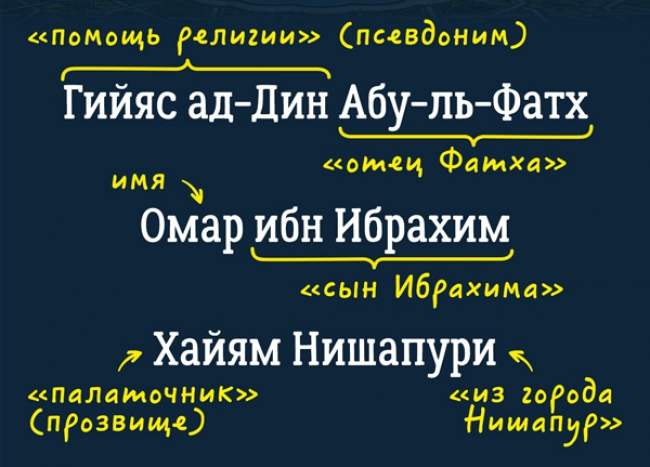
\includegraphics[width=0.7\linewidth]{img/haiyam}
    \caption{Расшифровка полного имени \emph{Омара Хайяма}}
    \label{fig:haiyam}
\end{figure}

\section{Китайские имена}

\section{Тибетские имена}

Тибетская система им\"eн принципиально отличается от китайской и ориентирована в большей степени на Индию. В Тибете нет фамилий. Многие имена являются калькой с санскрита, но есть и традиционные (напр.: \emph{Дава} (тиб. \emph{луна, понедельник}), \emph{Ньима} (тиб. \emph{солнце, воскресенье})).

\emph{Джамьянг Шэпа} -- тибетский уч\"eный.

\section{Корейские имена}

Корейское имя состоит из фамилии и следующего после него личного имени.

В большинстве случаев фамилия состоит из одного слога, а имя из двух слогов. Как имя, так и фамилия часто записываются с помощью \emph{ханча} -- китайских иероглифов, отражающих корейское произношение. Ханча более не используются в Северной Корее, а их использование для имён в Южной Корее сокращено до 5038 иероглифов. При использовании европейских языков некоторые корейцы сохраняют традиционный порядок написания, а другие меняют его согласно западной схеме.

В Корее используется всего около 250 фамилий. Самыми распространёнными из них являются \emph{Ким}, \emph{Ли} и \emph{Пак}. Однако большинство однофамильцев не являются близкими родственниками. Происхождение корейских фамилий тесно связано с корейской историей и географией.

\emph{Ким Дон Ин} -- корейский писатель.

\emph{Ким Юджон} -- корейский писатель.

\emph{Пак Кю Су} -- корейский государственный деятель и писатель.

% TODO Японские имена

% TODO Индийские имена

\section{VIAF}

Для выяснения форм написания имени и фамилии рекомендуется использовать сайт \underline{http://viaf.org} (англ. \emph{Virtual International Authority File} — виртуальный международный авторитетный файл) -- виртуальный каталог международного нормативного контроля (информации о произведениях и их авторах). В разработке проекта участвовало несколько крупнейших мировых библиотек, в том числе Немецкая национальная библиотека, Библиотека Конгресса США и РНБ.

\begin{figure}
    \centering
    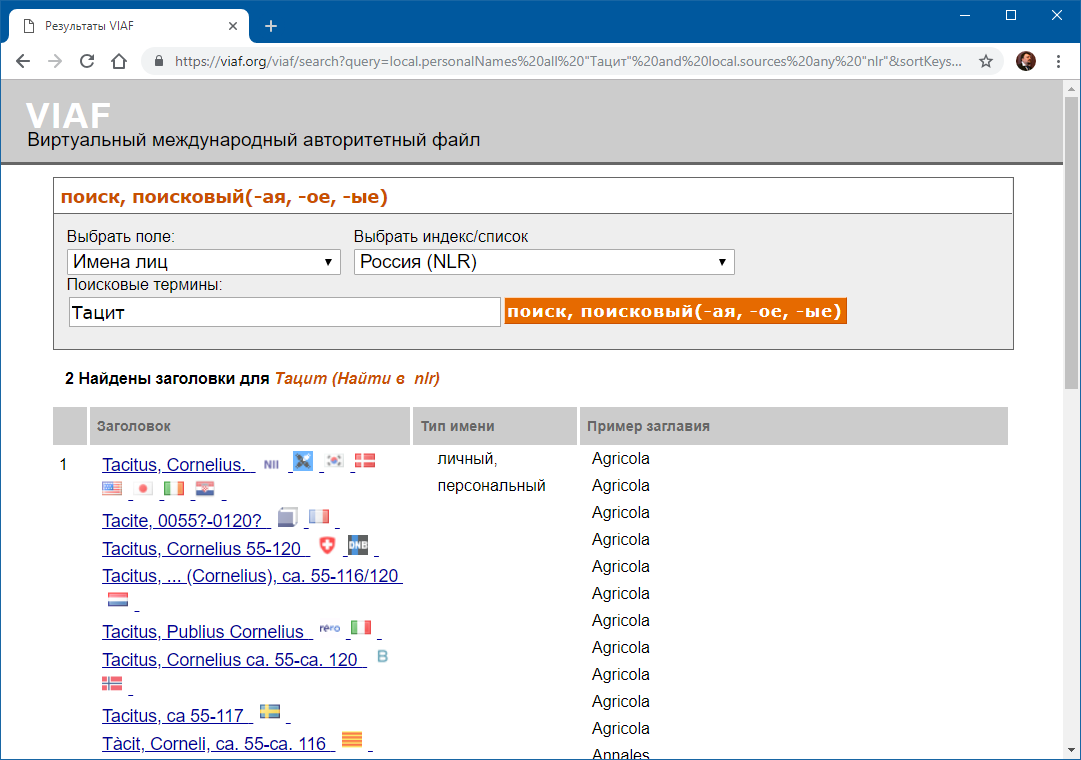
\includegraphics[width=\linewidth]{img/viaf}
    \caption{Сайт VIAF}
    \label{fig:viaf}
\end{figure}


\chapter{Поля 70x: индивидуальные авторы}

Блок полей 7xx в RUSMARC  -- блок ответственности, он содержит имена лиц и наименования организаций, надел\"eнных той или иной степенью ответственности по отношению к каталогизируемому документу (создание документа, его распространение, владение документом и т.п.).

Ответственность подразделяется на первичную и вторичную. Первичную ответственность могут нести одно лицо, одна организация или один род / династия / семья. Другие лица, роды / династии / семьи, организации, несущие равную с ними ответственность, наделены статусом альтернативной ответственности.

Если основной точкой доступа в записи является заглавие, лица, роды / династии / семьи и организации могут быть наделены статусом альтернативной или вторичной ответственности: авторы (один или несколько авторов с равной степенью ответственности) наделяются статусом альтернативной ответственности; редакторы, переводчики, авторы иллюстраций и т.д. -- статусом вторичной ответственности.

Если невозможно определить уровень ответственности, все лица и организации рассматриваются как несущие вторичную ответственность.

При внесении сведений в данное поле основным моментом является определение фамилии автора или первого элемента при ее отсутствии. Имя автора приводится в форме, получившей наибольшую известность. В качестве ориентира здесь должны выступать энциклопедические словари, справочники и национальный авторитетный файл.

\section{Подполе A: фамилия}

\section{Подполе B: инициалы}

\section{Подполе G: расширение инициалов}

\section{Подполе 9: роль (инвертирование ФИО допустимо?)}

Устанавливается в значение \emph{1} (соответствует положению переключателя \emph{Отменить умолчание}), если имя записано в прямом порядке.

Имя записано в прямом порядке:

\begin{cutelist}
    \item ИМЯ;
    \item ИМЯ ОТЧЕСТВО;
    \item ИМЯ ПРОЗВИЩЕ (ЭПИТЕТ, ОПРЕДЕЛЕНИЕ);
    \item ИМЯ [ФАМИЛИЯ ИМЯ ОТЧЕСТВО] ДУХОВНОЕ ЗВАНИЕ;
    \item ИМЯ ИМЯ ИМЯ (китайские и другие восточные имена);
    \item СОКРАЩЕННОЕ ИМЯ (.) ИНИЦИАЛ;
    \item ИНИЦИАЛ (.) СОКРАЩЕННОЕ ИЛИ ПОЛНОЕ ИМЯ.
\end{cutelist}

Имя записано под фамилией, родовым именем, отчеством:

\begin{cutelist}
    \item ФАМИЛИЯ (,) ИМЯ ОТЧЕСТВО (то же в инициальной форме);
    \item ФАМИЛИЯ (,) ИМЯ (то же инициалы);
    \item ФАМИЛИЯ;
    \item ФАМИЛИЯ (-) ФАМИЛИЯ (,) ИМЯ ОТЧЕСТВО (то же в инициальной форме);
    \item ФАМИЛИЯ ФАМИЛИЯ ФАМИЛИЯ (,) ИМЯ (то же инициалы);
    \item СОКРАЩЕННАЯ ФАМИЛИЯ (,) ИМЯ (то же инициалы).
\end{cutelist}

Если имя приведено в прямом порядке, то в подполях 9 и L должно быть установлено значение \emph{1}, а подполя B и G должны быть пустыми.

Заполнение подполя 9 влияет на автоматическое формирование сведений об ответственности. В частности, если установить его в \emph{1}, то в сформированных сведениях об ответственности инициалы будут помещены после фамилии автора. Поэтому, если на титульном листе ФИО автора приведено как \emph{Иванов А. А.}, то подполе 9 следует установить в \emph{1}.

\section{Подполе 1: неотъемлемая часть имени}

Неотъемлемая часть имени -- та, которая не может измениться в течение жизни. Если часть имени может измениться, то она не является неотъемлемой и заносится в подполе C.

\textbf{Примеры.}

\begin{cutelist}
    \item барон;
    \item младший;
    \item отец;
    \item святитель;
    \item сын;
    \item Jr.
\end{cutelist}

\textbf{Типичные ошибки.}

\begin{cutelist}
    \item диакон;
    \item д-р, профессор Гейдельбергского университета;
    \item оглы;
    \item писатель, общественный деятель.
\end{cutelist}

\section{Подполе C: дополнения к именам, кроме дат}

Любые дополнения к именам (кроме дат), которые не являются неотъемлемой частью имени (титулы, звания, эпитеты, указание должности).

Допускаются сокращения по ГОСТ.

\textbf{Примеры.}

\begin{cutelist}
    \item доктор биологических наук, профессор;
    \item заслуж. учитель РСФСР, канд. пед. наук;
    \item чемпион мира по шахматам (1975-1985).
\end{cutelist}

\textbf{Типичные ошибки.}

\begin{cutelist}
    \item Димитр Христов Чорбаджийский;
    \item Епископ Диоклийский Каллист (Уэр);
    \item лорд;
    \item отец ; французский писатель.
\end{cutelist}

% TODO Шаблоны дополнения

\section{Подполе L: индикатор формы записи имени}

Подполе устанавливается в значение \emph{1} (соответствует положению переключателя \emph{Отменить умолчание}), если в подполе A введена не фамилия, а другой элемент имени.

Если в подполе L установлено значение \emph{1}, то подполя B и G должны быть пустыми.

\section{Подполе D: римские цифры}

Римские цифры, связанные с именами римских пап, членов королевских семей и священнослужителей. Если имеется эпитет (второе имя, прозвище и т.п.), связанный с нумерацией, эпитет также включается в подполе D. При использовании подполя D индикатор -- подполе 9 -- обязательно должен быть пустым.

\textbf{Примеры:}

\begin{cutelist}
    \item \textbf{\^{}A}Петр\textbf{\^{}D}II Карагеоргиевич\textbf{\^{}C}король югославский\textbf{\^{}F}1923-1970\textbf{\^{}9}1
    \item \textbf{\^{}A}Иван\textbf{\^{}C}князь московский\textbf{\^{}D}I Данилович Калита\textbf{\^{}F}ок. 1288-1340
\end{cutelist}

\section{Подполе F: даты жизни}

Даты, присоединяемые к именам лиц, включая слова, указывающие на смысл дат (например, жил, родился, умер). Указанные слова вводятся в подполе в полной или сокращенной форме. Все даты для лица, названного в поле, вводятся в одно подполе F.

Диапазон дат вводится через дефис без пробелов.

Век приводится в числовом виде в арабской нотации. Для веков до нашей эры обязательно указывается "<до н. э.">.

Приблизительные даты приводятся со словом «около».

Даты, вызывающие сомнения (установленные по недостоверным источникам), приводятся со знаком вопроса.

У ныне живущих авторов вводится дата рождения, дефис и пробел.

\textbf{Примеры.}

\begin{cutelist}
    \item 1618-1693
    \item 1797 или 1798-1871
    \item около 1048-после 1122
    \item 1978-
    \item 2 в. до н. э.
    \item 1258-?
\end{cutelist}

\textbf{Типичные ошибки.}

\begin{cutelist}
    \item 712 -- 770
    \item V в. н. э.
    \item 11-й в.
\end{cutelist}

\section{Подполе R: разночтение фамилии}

В подполе R "<Разночтение фамилии"> вводится вместе с инициалами псевдонимы или подлинные имена авторов (в зависимости от того, какое имя было внесено в подполе A "<Фамилия">) выводится в поисковый словарь авторов (наряду с основным именем), и на него готовится ссылочная каталожная карточка.

Применяется одна из тр\"eх схем:

\begin{cutelist}
    \item Имя в прямой форме
    \item Фамилия И. О.
    \item Фамилия, Имя Отчество
\end{cutelist}

\textbf{Примеры.}

\begin{cutelist}
    \item Августин Блаженный
    \item Б. Г.
    \item Ло Хуа-шэн
    \item Низами Гянджеви Абу Мухаммед Ильяс ибн Юсуф
    \item Фон-Визин
    \item Чхартишвили, Григорий Шалвович
\end{cutelist}

\textbf{Типичные ошибки.}

\begin{cutelist}
    \item Екатерина Мечиславовна Насута
    \item Полное имя: Феликс Лопе де Вега и Карпио
    \item Элизабет Роузмонд Тейлор
    \item Эффос, А. Э.
\end{cutelist}

\section{Подполе Y: работает в данной организации}

Переключатель "<Да/Нет">.
Устанавливается в "<Да">, если автор работает в настоящее время (или работал на момент публикации документа) в организации, создающей библиографическое описание.

\section{Подполе P: место работы автора}

Организационно-правовые формы в наименовании организации опускаются.

\textbf{Примеры.}

\begin{cutelist}
    \item Клуб бухгалтеров и аудиторов некоммерческих организаций
    \item Московский государственный университет культуры и искусств
    \item Российский государственный торгово-экономический университет
\end{cutelist}

\textbf{Типичные ошибки.}

\begin{cutelist}
    \item Главный научный сотрудник Отдела взаимосвязей русской и зарубежных литератур Института русской литературы (Пушкинский Дом) РАН
    \item НОУ "Тольяттинская академия управления"
\end{cutelist}

\section{Подполя 4, 5, 6: функция}

Функции лиц со вторичной ответственностью заполнять строго с помощью встроенного меню, не добавляя пояснений вроде "<730 пер. с фр."> После того, как АРМ автоматически сформирует сведения об ответственности, привести их к соответствию с предписанным источником путем редактирования.

Недопустимо вводить две и более функции в одном подполе (например, "<070 авт. и ред.">). Выбирается одна, первая, функция, затем автоматически сформированные сведения об ответственности редактируются вручную для приведения в соответствие с предписанным источником информации.

Соответствие нестандартных функций.

\begin{center}
\begin{tabular}{|l|l|}
    \hline 
    \thead{Нестандартная функция} & \thead{Стандартная функция}  \\ 
    \hline 
    Подготовка текста & 340 редактор  \\ 
    \hline 
    Научная подготовка текста & 340 редактор  \\ 
    \hline 
    Текст &  570 без расшифровки \\ 
    \hline 
    Автор-составитель & 220 составитель \\ 
    \hline 
\end{tabular}
\end{center}

Часто встречаются книги, в которых составитель на титульном листе оформлен как автор, а на обороте титульного листа или в тексте четко обозначено, что он является составителем или переводчиком. В качестве примера: стихи А.~С.~Пушкина в переводе на эвенкийский язык, переводчик В. Кейметинов на титульном листе оформлен как автор (над заглавием). В соответствии с договоренностью между РГБ и РНБ было принято решение следовать за формальными признаками -- оформлением титульного листа. В вышеприведенном примере книга будет оформлена под автором Кейметинов, а Пушкин станет соавтором. В поле 327 "<Примечания о содержании"> будет записано "<Стихи А. С. Пушкина в переводе В. Кейметинова">.

\chapter{Поля 710x: коллективные авторы}


\section*{Поле 200: основное заглавие}

Блок 2xx в RUSMARC -- блок описательной информации, он содержит данные для всех областей описания ISBD, кроме Области примечания и Области стандартного номера (или его альтернативы) и условий доступности стандартов ISBD и ГОСТ 7.1-2003. 

\chapter{Поле 205: сведения об издании}

ГОСТ 7.1-2003, п. 5.3

Поле повторяется (например, в случае ошибочного указания издания).

Содержит информацию об изменениях и особенностях данного издания по отношению к предыдущему изданию того же произведения.

\section*{Подполе A: сведения об издании}

Содержит: сведения (слово, фраза или группа символов), имеющиеся в пред-писанном источнике информации, либо сформулированные каталогизатором в соответствии с Правилами, и идентифицирующие документ с точки зрения издания.

Следует использовать встроенный справочник \textit{205.mnu}.

Номер издания следует приводить в цифровой форме в арабской нотации с наращением окончания числительного, независимо от того, в какой форме оно приведено в предписанном источнике информации.

\chapter{Поле 210: выходные данные}

Соответствует полю RUSMARC: 210

ГОСТ 7.1-2003, п. 5.5

Повторяется для каждого издательства.

ГОД ИЗДАНИЯ (подполе d) — последний элемент выходных данных издания. Им по закону РФ "Об авторском праве и смежных правах" от 09.07.1993 N 5351-1 считается год выпуска в обращение экземпляров произведения (издания), т. е. год сдачи тиража или его начальной партии книготорговцу. Указывается арабскими цифрами (без сокращенного или полного слова "год". ГОСТ 7.4—95 требует в повторных изданиях проставлять на обороте титульном листе год выпуска предшествующего издания (напр.: 2-е издание вышло в 1975 г.), а в многотомных -- год выпуска первого тома, т. е. начала выпуска всего многотомного издания (напр.: Т. 1 вышел в 1991 г.), однако при контртитуле с общими для всего многотомного издания выходными сведениями целесообразно в выходных данных ставить год выпуска 1-го тома с висячим тире во всех томах, кроме последнего, где указывают год выпуска первого тома и через тире -- последнего.

В периодических (кроме газет) и продолжающихся изданиях год издания указывают при номере издания независимо от года выхода его в свет.

\chapter*{Поле 215: количественные характеристики}

ГОСТ 7.1-2013, п. 5.6

Повторяется для разных физических носителей.

Если в подполе "Объем" 215\^{}a используется двойная (тройная) пагинация, надо использовать справочник-меню.

Подполе "Единица измерения" 215\^{}1 не должно содержать "с." или "л.".

\chapter{Поле 101: язык основного текста}

Поле обязательное.

Повторяемое. Повторяется для каждого языка, используемого в тексте.

Коды языков всегда вводятся строчными латинскими буквами, состоят из трех символов и берутся строго из встроенного справочника \emph{jz.mnu}!

Первым указывается язык, применяемый в данном документе в наибольшей степени. При неоднозначности (непонятно, какой из двух языков основной для документа) рекомендуется использовать код русского языка \emph{rus}, если, конечно, в документе имеется русский язык.

Небольшие цитаты (объёмом не более одного абзаца) не учитываются!

Для многоязычных документов (более 3 языков) можно использовать код языка \emph{mul} – "<мультиязычный документ">.

Для документов, язык которого определить невозможно (в том числе по причине отсутствия письменного текста и/или аудиосопровождения), нужно ис-пользовать код \emph{und} – <"не определено">.

Нельзя использовать вместо трехбуквенного кода языка двухбуквенный код страны.

\chapter*{Поле 102: страна}

Поле обязательное.

Повторяемое. Повторяется для каждой из стран, в которой издавался документ.

Перечень названий стран и их коды по ГОСТ 7.67-2003, введенному в действие 1 января 2005 года.

Постановлением Госстандарта РФ от 14 декабря 2001 г. N 529-ст)(с изменениями N 1/2003, 2/2003, 3/2004, 4/2004, 5/2005) в 2001 г. при-нят введён в действие Общероссийский классификатор стран мира OK (MK (ИСО 3166) 004-97) 025—2001 (ОКСМ).

Коды стран всегда вводятся прописными латинскими буквами, состоят из двух символов и берутся строго из встроенного справочника str.mnu!

Первой указывается… % TODO дописать

Заполняется строго значениями из справочника!

Если в справочнике отсутствует код страны, в которой был издан документ, то используется код страны, исторически последующей.

\chapter{Поле 10: ISBN, цена}

ГОСТ 7.1-2003, п. 5.9 % TODO Ссылка на новый ГОСТ

Поле повторяется для нескольких ISBN одного издания.
 
Вопросы, связанные с Международным стандартным книжным номером (ISBN) регулируются ГОСТ 7.0.53-2007.

ISBN действующего стандарта состоит из тринадцати цифр, поделенных на пять групп, разделяемых знаком дефиса.

\begin{enumerate}
    \item Префикс EAN.UCC -- код \emph{978} (в дальнейшем будет использоваться \emph{979}), предоставленный Европейской ассоциацией товарной нумерации (EAN) Международному агентству ISBN для обозначения товара "<Книжная продукция">.
    \item Номер регистрационной группы служит для обозначения в ISBN страны, географической или языковой области. Для Российской Федерации номер регистрационной группы -- цифра \emph{5}.
    \item Номер регистранта идентифицирует в системе ISBN конкретного издателя, производителя документов. Номер регистранта российский издатель (производитель документов) получает в Российском национальном агентстве ISBN, функционирующем в составе Российской книжной палаты.
    \item Номер издания (публикации) идентифицирует конкретное издание (публикацию) издателя, производителя документов в предоставленном ISBN.
    \item Контрольная цифра служит для проверки правильности цифровой части ISBN.
\end{enumerate}

ISBN старого стандарта состоял из десяти цифр, поделенных на четыре группы, -- в нем не было префикса EAN, остальные группы совпадают с действующим стандартом.

\textbf{Примеры.}

\begin{cutelist}
	\item 0-812-57558-X \emph{(старый стандарт)};
	\item 5-02-003157-7;
	\item 978-5-98846-049-7 \emph{(действующий стандарт)}.
\end{cutelist}

В издании, выпущенном совместно несколькими издателями (в том числе, российскими и зарубежными издателями) приводят ISBN каждого издателя-партнера. Наименование издателя указывают после соответствующего ISBN в круглых скобках без кавычек в той форме, как оно приведено на титульной странице.

\textbf{Примеры.}

\begin{cutelist}
	\item 978-5-09-014485-8 (Просвещение);
	\item 978-5-472-01012-2 (Экзамен);
	\item 978-1 -84334-151-2 (Chandos Publishing);
	\item 978-5-93913-059-3 (Профессия).
\end{cutelist}

В томе (выпуске) многотомного издания приводят ISBN данного тома (с указанием в круглых скобках обозначения и номера тома) и ISBN многотомного издания в целом.

\textbf{Пример.}

\begin{cutelist}
	\item ISBN 978-5-02-033899-9 (т. 1);
	\item ISBN 978-5-02-033897-5.
\end{cutelist}

В издании, входящем в состав комплектного, комбинированного издания, приводят ISBN данного издания (с указанием в круглых скобках сведений "<отд. кн."> или "<отд. изд.">) и ISBN комплектного, комбинированного издания в целом.

\textbf{Пример.}

\begin{cutelist}
	\item 978-5-89349-822-6 (отд. кн.)
	\item 978-5-89349-820-2
\end{cutelist}

ISBN комплектного комбинированного издания в целом приводят на футляре, папке, обложке комплектного издания.

В поле вводятся только ISBN, относящиеся непосредственно к обрабатываемому документу. Прочие ISBN, относящиеся, например, к электронной версии или к изданию в твердом переплете, опускаются. Также опускается ISBN, относящийся к многочастному документу в целом.
Если невозможно определить, какой ISBN к чему относится, то приводят все имеющиеся ISBN (ГОСТ 7.1-2003, п. 5.9.2). % TODO ссылка на новый ГОСТ

\section{Подполе A: ISBN}

Подполе имеет ФЛК, проверяющее правильность написания ISBN по контрольной цифре и сверяющее его на дублетность. Контроль не блокирующий, при наличии ошибок можно продолжать ввод и сохранять запись.

\textbf{Типичные ошибки.}

\begin{cutelist}
    \item употребление кириллической буквы Х вместо латинской X;
    \item употребление пробелов вместо дефисов в качестве разделителя групп;
    \item запись ISBN без разделителей;
    \item ввод уточняющих сведений, которые должны быть внесены в подполе B.
\end{cutelist}

\section{Подполе B: уточнения}

\textbf{Примеры.}

\begin{cutelist}
    \item Бином
    \item Кн. 1
    \item в пер.
\end{cutelist}

Типичная ошибка: ввод сведений в скобках.

\section{Подполе Z: ошибочный ISBN}

Подполе Z отличается от подполя A отсутствием ФЛК. Сюда нужно вносить ISBN, про которые точно известно, что они ошибочные.

\section{Подполе D: общая для всех экземпляров цена}

\textbf{Примеры.}

\begin{cutelist}
    \item 1.00
    \item 1000.00
    \item 123.45
\end{cutelist}

\textbf{Типичные ошибки.}

\begin{cutelist}
    \item 5 руб.
    \item 10 коп.
    \item 10,50
    \item 12
\end{cutelist}

\section{Подполе C: обозначение валюты}

\textbf{Примеры.}

\begin{cutelist}
    \item Fr
    \item USD
    \item тенге
\end{cutelist}

\textbf{Типичные ошибки.}

\begin{cutelist}
    \item руб.
    \item \$
\end{cutelist}

\chapter{Поля 461 и 46: общие сведения для многотомника}

Съешь ещё этих мягких французских булок, да выпей, дружок, чаю. В чащах юга жил-был цитрус, но фальшивый экземпляр. Съешь ещё этих мягких французских булок, да выпей, дружок, чаю. В чащах юга жил-был цитрус, но фальшивый экземпляр. Съешь ещё этих мягких французских булок, да выпей, дружок, чаю. В чащах юга жил-был цитрус, но фальшивый экземпляр.

Съешь ещё этих мягких французских булок, да выпей, дружок, чаю. В чащах юга жил-был цитрус, но фальшивый экземпляр. Съешь ещё этих мягких французских булок, да выпей, дружок, чаю. В чащах юга жил-был цитрус, но фальшивый экземпляр. Съешь ещё этих мягких французских булок, да выпей, дружок, чаю. В чащах юга жил-был цитрус, но фальшивый экземпляр.

Съешь ещё этих мягких французских булок, да выпей, дружок, чаю. В чащах юга жил-был цитрус, но фальшивый экземпляр. Съешь ещё этих мягких французских булок, да выпей, дружок, чаю. В чащах юга жил-был цитрус, но фальшивый экземпляр. Съешь ещё этих мягких французских булок, да выпей, дружок, чаю. В чащах юга жил-был цитрус, но фальшивый экземпляр.
\chapter*{Поле 300: общие примечания}

Соответствует полю RUSMARC: 300

ГОСТ 7.1-2003, п. 5.8

Повторяется. Если вводится более одного примечания, каждое вводится в новое повторение поля.

Содержит дополнительную информацию об объекте описания, которая не была приведена в других элементах описания. Сведения, приводимые в поле, заимствуют из любого источника и в квадратные скобки не заключают.

Слова текста, заключенные в угловые скобки < >,  включаются в словарь ключевых слов.

\textbf{Примеры.}

\begin{itemize}
	\item В надзаг.: Посвящается 60-летию Уфимского государственного нефтяного технического университета
	\item Деп. в ВИНИТИ 18.05.02, № 14432
	\item Издание выходило полутомами с последовательной нумерацией выпусков на корешках переплета
	\item Лауреат конкурса «Профессиональный учебник»
	\item На корешке указан том серии
	\item На шмуцтитуле: «Издано под наблюдением Комиссии при Комитете состоящего под высочайшим государя императора покровительством Императорского Общества любителей древней письменности»
	\item Посвящается памяти академика Д. С. Белянкина
	\item Продолжение романа «Ветер над полем»
	\item Произведение печатается без сокращений
	\item Электронные версии книг на сайте www.prospeckt.org
\end{itemize}

\textbf{Типичные ошибки.}

\begin{itemize}
	\item (Библиотека детского романа)
	\item (На обл: Опыт передового учителя)
	\item Авторы указаны на обороте тит. л. - Библиогр.: с. 287 (9 назв.).
	\item Загл. корешка: Великий Октябрь и реальный социализм
	\item Часть текста: англ.
\end{itemize}


\chapter*{Поле 314: примечания об интеллектуальной ответственности}

Не повторяется.

\textbf{Примеры.}

\begin{itemize}
	\item Авторы указаны в оглавлении;
	\item Авторы указаны на обороте титульного листа;
	\item Заглавие с этикетки видеодиска;
	\item Сведения об авторах: с. 693-698.
\end{itemize}

\textbf{Типичные ошибки.}

\begin{itemize}
	\item Книга фактически издана в 2012 г.;
	\item Указ. имен и ил.: с. 415-424;
	\item Писательница Серова Марина -- это не реальный человек, а многочисленный коллектив авторов из Саратова, работающих под руководством одного литературного агента;
	\item Ранее кн. выходила под назв. «Адская смесь».
\end{itemize}

\chapter*{Поле 225: область серии}

ГОСТ 7.1-2003, п. 5.7

Поле содержит заглавие серии вместе с любыми сведениями, относящимися к этому заглавию, и сведениями об ответственности, относящимися к заглавию серии.

Повторяется, если документ входит более чем в одну серию.

\section*{Подполе A: Наименование}

Заглавие серии в той форме, в которой оно представлено в источнике информации.

Подполе обязательное.

\textbf{Примеры.}

\begin{itemize}
	\item Библиотечка автомобилиста;
	\item За Родину! За Победу!
	\item Классики мировой психологии
\end{itemize}

\textbf{Типичные ошибки.}

\begin{itemize}
	\item Серия "Высшее образование"
\end{itemize}

\section*{Подполе V: Обозначение и Номер выпуска в серии}

Номер каталогизируемого документа внутри серии.

\textbf{Примеры.}

\begin{itemize}
	\item Вып. 22
	\item Кн. 6
	\item Т. 40	
\end{itemize}

\textbf{Типичные ошибки.}

\begin{itemize}
	\item Вып. № 22
	\item Малая серия
	\item Т. CXXVII
\end{itemize}

\chapter*{Заключение}

Съешь ещё этих мягких французских булок, да выпей, дружок, чаю. В чащах юга жил-был цитрус, но фальшивый экземпляр. Съешь ещё этих мягких французских булок, да выпей, дружок, чаю. В чащах юга жил-был цитрус, но фальшивый экземпляр. Съешь ещё этих мягких французских булок, да выпей, дружок, чаю. В чащах юга жил-был цитрус, но фальшивый экземпляр.

Съешь ещё этих мягких французских булок, да выпей, дружок, чаю. В чащах юга жил-был цитрус, но фальшивый экземпляр. Съешь ещё этих мягких французских булок, да выпей, дружок, чаю. В чащах юга жил-был цитрус, но фальшивый экземпляр. Съешь ещё этих мягких французских булок, да выпей, дружок, чаю. В чащах юга жил-был цитрус, но фальшивый экземпляр.

Съешь ещё этих мягких французских булок, да выпей, дружок, чаю. В чащах юга жил-был цитрус, но фальшивый экземпляр. Съешь ещё этих мягких французских булок, да выпей, дружок, чаю. В чащах юга жил-был цитрус, но фальшивый экземпляр. Съешь ещё этих мягких французских булок, да выпей, дружок, чаю. В чащах юга жил-был цитрус, но фальшивый экземпляр.

\backmatter

\chapter{Примеры библиографических описаний}

Съешь ещё этих мягких французских булок, да выпей, дружок, чаю. В чащах юга жил-был цитрус, но фальшивый экземпляр. Съешь ещё этих мягких французских булок, да выпей, дружок, чаю. В чащах юга жил-был цитрус, но фальшивый экземпляр. Съешь ещё этих мягких французских булок, да выпей, дружок, чаю. В чащах юга жил-был цитрус, но фальшивый экземпляр.

Съешь ещё этих мягких французских булок, да выпей, дружок, чаю. В чащах юга жил-был цитрус, но фальшивый экземпляр. Съешь ещё этих мягких французских булок, да выпей, дружок, чаю. В чащах юга жил-был цитрус, но фальшивый экземпляр. Съешь ещё этих мягких французских булок, да выпей, дружок, чаю. В чащах юга жил-был цитрус, но фальшивый экземпляр.

Съешь ещё этих мягких французских булок, да выпей, дружок, чаю. В чащах юга жил-был цитрус, но фальшивый экземпляр. Съешь ещё этих мягких французских булок, да выпей, дружок, чаю. В чащах юга жил-был цитрус, но фальшивый экземпляр. Съешь ещё этих мягких французских булок, да выпей, дружок, чаю. В чащах юга жил-был цитрус, но фальшивый экземпляр.
\chapter{Клавиатурные сокращения}

%\noindent\begin{longtable}{|>{\raggedright } p{7.5cm} |>{\raggedright } p{3cm} |}
\noindent\begin{longtable}{| p{7.5cm} | p{3cm} |}
	\hline
	\thead{Действие} & \thead{Клавиши} \\
	\hline\endfirsthead
	\thead{Действие} & \thead{Клавиши} \\
    \hline\endhead
    \hline
    \multicolumn{2}{c}{\emph{Продолжение на следующей странице}}   \\
    \endfoot
    \hline\endlastfoot
     Восстановление исходного значения поля, отказ от редактирования & Esc \\
	\hline
	Переход к следующему полю или подполю & Enter или $\downarrow$ \\
	\hline
	Новое повторение поля & Ctrl + $\downarrow$ \\
	\hline
	Переключение между вкладками рабочей области & Ctrl + $\rightarrow$ или $\leftarrow$ \\
	\hline
	Переход в конец страницы ввода & Page Down \\
	\hline
	Переход в начало страницы ввода & Page Up \\
	\hline
	Вызов вложенного рабочего листа, словаря или средства ввода & F2 \\
	\hline
	Мультиввод (повторения поля в виде таблицы) & F3 \\
	\hline
	Оперативное меню: сокращения по ГОСТ 7.12-93 и ГОСТ Р 7.0.12-2011, римские цифры, коды языков, команды контекстного выделения & F4 \\
	\hline
	Исправление кириллических символов, ошибочно набранных латиницей & F6 \\
	\hline
	Исправление символов, ошибочно введ\"eнных в верхнем регистре (с включенным Caps Lock) & F7 \\
	\hline
	Сохранение записи & Shift + Enter \\
	\hline
	Создание новой записи & Alt + Плюс на цифровой клавиатуре \\
	\hline
	Ввод текущей даты & Alt + Д \\
	\hline	
	Переход к первой записи & Shift + Page Up \\
	\hline
	Переход к последней записи & Shift + Page Down \\
	\hline
	Переход к следующей записи & Shift + $\downarrow$ \\
	\hline
	Переход к предыдущей записи & Shift + $\uparrow$ \\
	\hline
	Выход из вложенного рабочего листа, словаря или средства ввода с сохранением ввода & Tab, затем Enter \\
	\hline
	Выход из вложенного рабочего листа, словаря или средства ввода с отменой внесенных изменений & Последовательность Tab-Tab-Enter \\
	\hline
	Виртуальная клавиатура & Alt + V \\
	\hline
	Виртуальная клавиатура языковая & Alt + K (латинская) \\
	\hline
	Импорт из ЛИБНЕТ & Alt + I \\
	\hline
	Импорт из ИРБИС-корпорации & Alt + W \\
	\hline
	Импорт из Z-ресурсов & Alt + Z \\
	\hline
\end{longtable}



% bibliography, glossary and index would go here.

\end{document}